\begin{theo}[Elektrische stroom]{Elektrische stroom}
    \textbf{Elektrische stroom} is het tempo waarmee er elektrische lading door een oppervlak stroomt. Het is dus eigenlijk een vorm van snelheid voor de lading. Voor een constant tempo bekomen we

    \begin{equation*}
        I_{gem} = \dfrac{\Delta Q}{\Delta t}
    \end{equation*} 
    
    \noindent en bij variërend tempo bekomen we

    \begin{equation*}
        I = \dfrac{dQ}{dt}
    \end{equation*} 
    De stroomzin is in de omgekeerde richting van de elektronenstroom,
    \begin{center}
        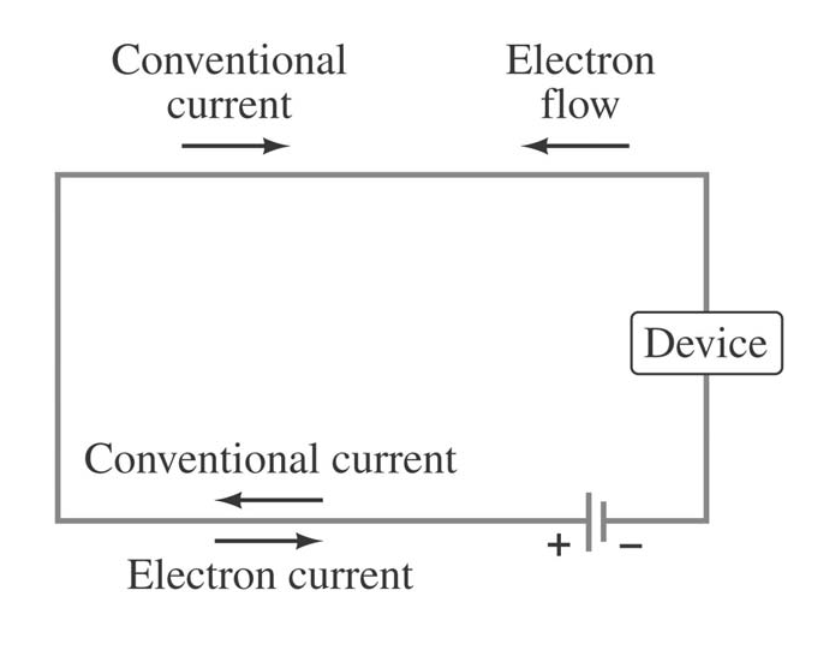
\includegraphics[scale = 0.4]{Images/Elektriciteit/Stroomzin.png}
    \end{center}
    maar wordt gedragen door de elektronen in metalen draden op microscopisch niveau en in fluïdum door protonen of elektronen. De stroomzin is dus eerder een conventie.
\end{theo}

\begin{app}[Microscopisch model van elektrische stroom]{Microscopisch model van elektrische stroom}
    We nemen aan dat we ons niet in het elektrostatisch geval bevinden, namelijk dat
    \begin{equation*}
        \Vec{E} \neq 0
    \end{equation*}
    en dus de ladingen vrij zijn om te bewegen. We definiëren nu een nieuwe microscopische grootheid, de stroomdichtheid $\Vec{J}$, die staat voor stroom per cross-sectionele oppervlakteeenheid: 
    \begin{equation*}
        I = \int \Vec{J} \cdot d\Vec{A}
    \end{equation*}
    Voor het uniforme geval krijgen we dus:
    \begin{equation*}
        J = \dfrac{I}{A}
    \end{equation*}
    \begin{center}
        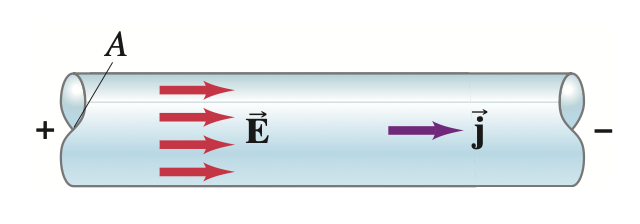
\includegraphics[scale = 0.5]{Images/Elektriciteit/MicroscopischStroom.png}
    \end{center}
    De richting van $\Vec{J}$ is gekozen volgens de stroomzin, maar in een geleider weten we dat de stroom gedragen wordt door de elektronen: ze bewegen dus eigenlijk in de met tegengestelde zin volgens $-\Vec{J}$. De elektronen voelen initieel een kracht door de aanwezigheid van het elektrisch veld en beginnen te versnellen. Hun versnelling in de tegengestelde zin van het elektrisch veld wordt de \textbf{driftsnelheid} genoemd. Deze is ongeveer gelijk omdat de elektronen constant botsen met de atomen van de draad en dus niet rechtstreeks bewegen volgens de elektronenstroom.
    \begin{center}
        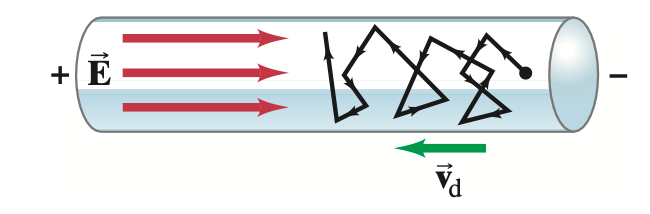
\includegraphics[scale = 0.53]{Images/Elektriciteit/Driftsnelheid.png}
    \end{center}
    Met deze nieuwe informatie kunnen we de voorgaande formules herschrijven, namelijk
    \begin{equation*}
        I = \dfrac{\Delta Q}{\Delta t} = \dfrac{n(-e)Av_d\Delta t}{\Delta t} = n(-e)Av_d
    \end{equation*}
    met $v_d$ de driftsnelheid: $\sim 10^{-4} m/s$, $-e$ de lading van een elektron en $n$ het aantal ladingen per volumeeenheid. De stroomdichtheid
    \begin{equation*}
        \Vec{J} = n(-e)\Vec{v_d} = \dfrac{n(-e)^2\tau}{m_e}\Vec{E}
    \end{equation*}
    met $\tau$ de gemiddelde tijd tussen 2 botsingen, heeft dus ook het minteken wat aanduid dat in werkelijkheid de stroomzin hier in de tegengestelde richting is van de driftsnelheid van de elektronen. De betekenis van weerstand op microscopisch niveau is het verlies van energie bij botsing tussen de elektronen en de atomen van de draad, want de vibraties zorgen voor de transformatie naar warmte.
\end{app}

\begin{theo}[Weerstand en resistiviteit]{}
    De grootte van de stroom is niet enkel afhankelijk van het potentiaal, maar ook van de \textbf{weerstand}. Het wordt gegeven door de volgende formule bij Ohmse materialen (zie hierna):
    \begin{equation*}
        R = \dfrac{\Delta V}{I} 
    \end{equation*}
    De \textbf{resistiviteit} $\rho$ van een draad 
    \begin{equation*}
        R = \rho \dfrac{l}{A}
    \end{equation*}
    is recht evenredig met de lengte $l$ en omgekeerd met de doorsnede. Het is afhankelijk van het materiaal van de draad en de temperatuur van de draad. Bij metalen groeit de resistiviteit lineair met de temperatuur, in formulevorm:
    \begin{equation*}
        \rho_T = \rho_0[1+\alpha(T-T_o)]
    \end{equation*}
    De \textbf{geleidbaarheid} van een materiaal kan men beschrijven door de inverse van de resistiviteit, ofwel:
    \begin{equation*}
        \sigma = \dfrac{1}{\rho}
    \end{equation*}
    \vspace{-0.5cm}
\end{theo}

\newpage

\begin{lem}[Ohm]{Ohm}
    De stroom doorheen een draad is recht evenredig met het potentiaalverschil over de twee uiteinden, in formulevorm:
    \begin{equation*}
         I \sim \Delta V
    \end{equation*}
    Ohm ontdekte ook dat bij metalen geleiders, zogenaamde `Ohmse' materialen,
    \begin{equation*}
         \Delta V= IR 
    \end{equation*}
    een constante bleek te zijn. Hieronder vergelijken we Ohmse materialen en niet-Ohmse materialen:
    \begin{center}
        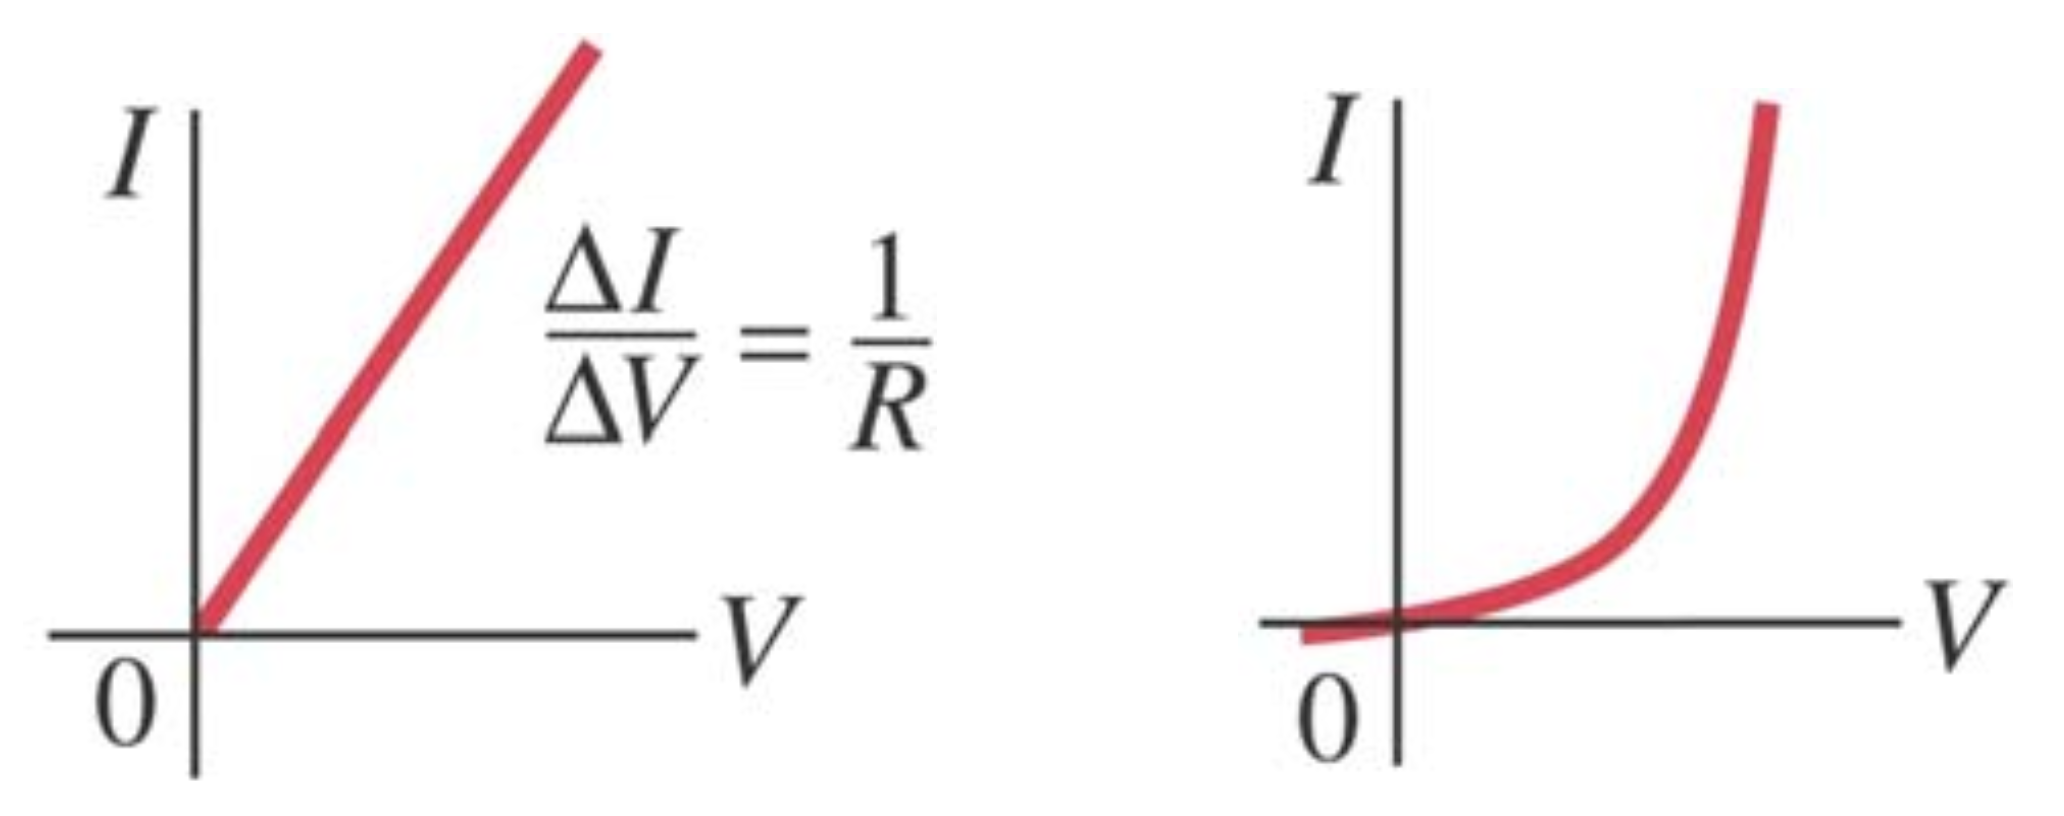
\includegraphics[scale = 0.2]{Images/Elektriciteit/GrafiekOhmseMaterialen.png}
    \end{center}
    Microscopisch zou dit betekenen dat de verhouding tussen de stroomdichtheid en het elektrische veld een constante, namelijk de \textbf{geleidbaarheid} van het materiaal, is, in formulevorm: 
    \begin{equation*}
        \Vec{J} = \sigma \Vec{E} \rightarrow \sigma = \dfrac{n(-e)^2\tau}{m_e}, \quad \rho = \dfrac{1}{\sigma} = \dfrac{m_e}{n(-e)^2\tau}
    \end{equation*}
\end{lem}

\begin{theo}[Elektrische Vermogen]{Elektrische Vermogen}
    We weten van voorgaande hoofdstukken dat vermogen een eenheid is voor arbeid per tijdseenheid: de mate waarin energie getransformeerd wordt. We vinden dus
    \begin{equation*}
        P = \dfrac{dU}{dt} = \dfrac{dq}{dt}\Delta V
    \end{equation*}
    en als we dit combineren met de definitie van stroom, bekomen we:
    \begin{equation*}
        P = I\Delta V
    \end{equation*}
    Deze formule kunnen we ook op andere manieren schrijven, namelijk:
    \begin{align*}
        P &=  I\Delta V= I(IR) = I^2R\\
        P &= I\Delta V = (\dfrac{\Delta V}{R})\Delta V = \dfrac{(\Delta V)^2}{R}
    \end{align*}
    Als we spreken over \textbf{supergeleidende} materialen, dan zijn deze volledig weerstandsloos en wordt er dus geen vermogen verloren aan warmte.
\end{theo}

% \begin{app}[Elektrische geleiding in metalen, isolatoren en halfgeleiders]{Elektrische geleiding in metalen, isolatoren en halfgeleiders}

% \end{app}

% \begin{app}[Halfgeleiders en doperen]{Halfgeleiders en doperen}

% \end{app}

% \begin{app}[Halfgeleiderdiodes]{Halfgeleiderdiodes}
    
% \end{app}

% \begin{app}[Transistoren en IC’s]{Transistoren en IC’s}
    
% \end{app}


